\documentclass[11pt,a4paper]{article}

\usepackage[utf8]{inputenc}
\usepackage[english]{babel}
\usepackage[T1]{fontenc}

\usepackage{amsmath,amssymb,amsfonts}
\usepackage{hyperref}

\usepackage{graphicx}
\usepackage{hyperref}

\title{Computational Geometry - Fortune's Algorithm}
\author{Philip Munksgaard \\ Sebastian Paaske Tørholm \\ Ejnar Håkonsen}

\begin{document}
\maketitle

\section{Exercise 7.4}
We wish to show that the break points of the beach line, $B$, trace out the Voronoi diagram, $Vor(P)$.

\begin{figure}[h!]
    \centering
    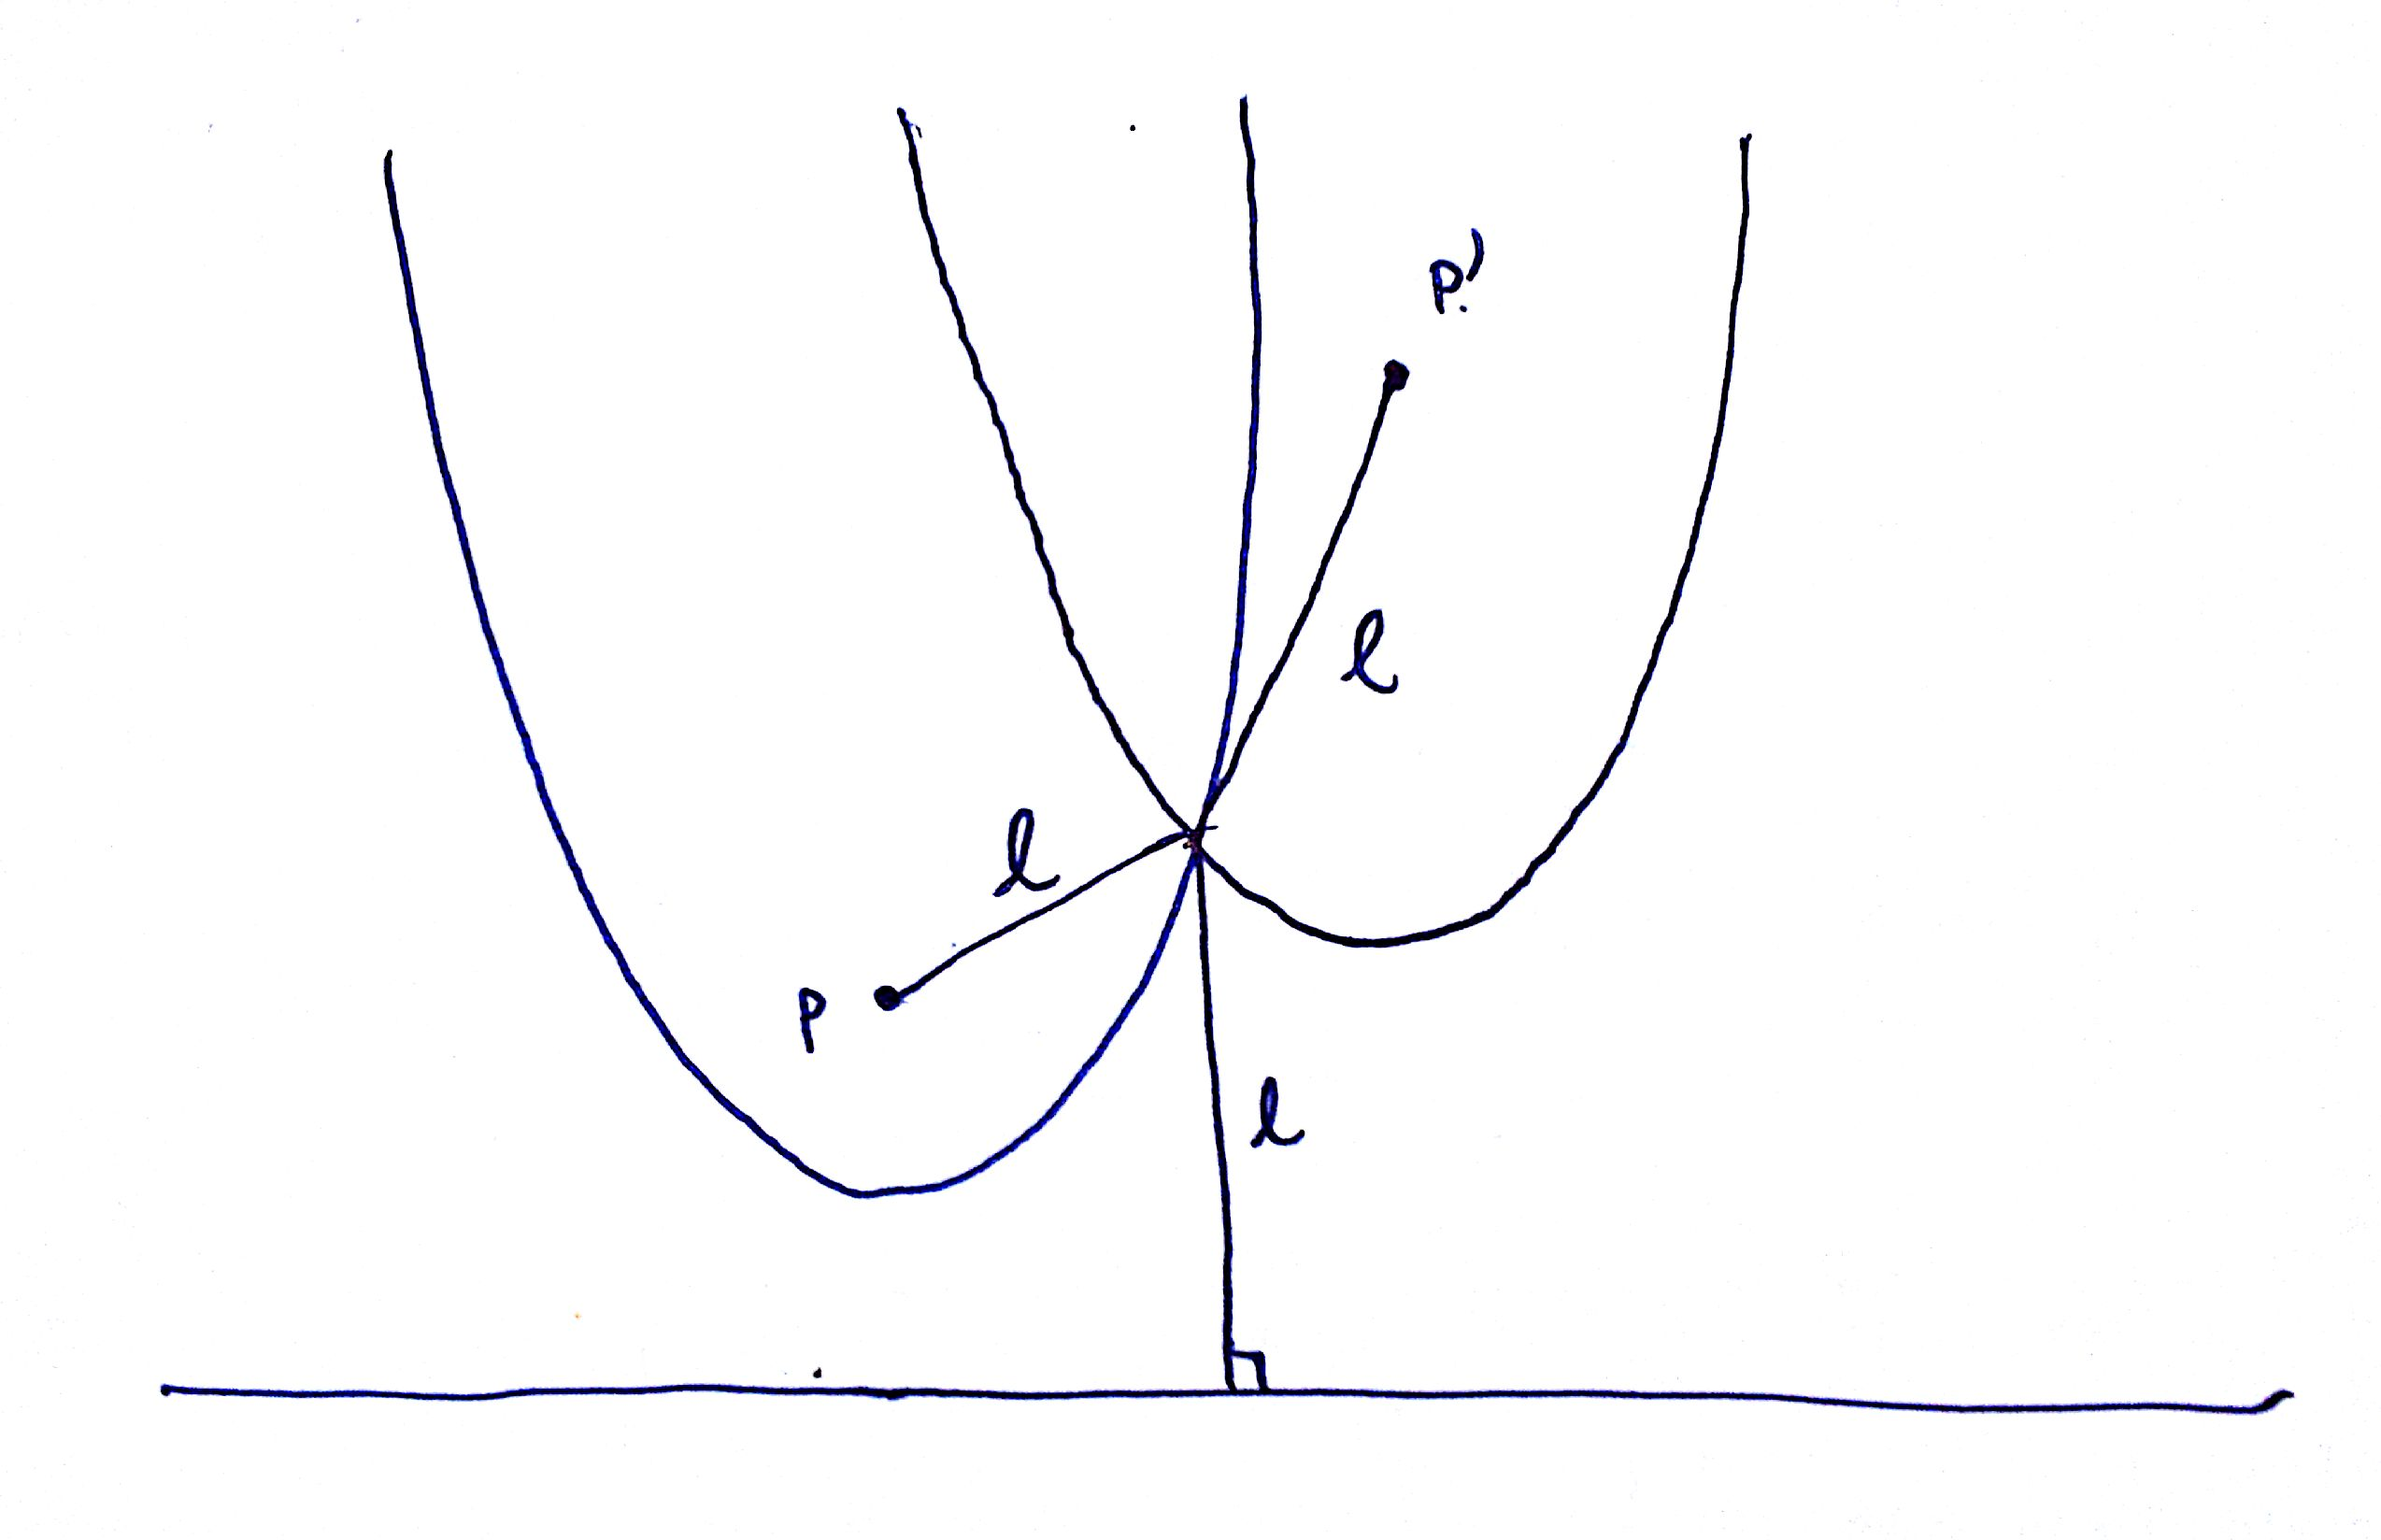
\includegraphics[width=.7\textwidth]{ex74-diagram.jpg}
    \caption{Distances between points, their parabolas, their intersection and the sweep line.}
    \label{ex74:dist}
\end{figure}

First we observe that each point in $B$ must be on the Voronoi diagram. We can
argue this by letting $b$ be such a break point. If the distance from $b$ to
the sweep line is $l$, then we must have that $p$ has distance $l$ to $b$, due
to $b$ being on its parabola. Likewise, $p'$ must also have distance $l$ to
$b$. As such, both points are equidistant to $b$. Since there are no
points closer to $b$ than $p$ and $p'$,\footnote{Since if there was, the
parabolas of $p$ and $p'$ wouldn't be on the beach line in $b$, as they would
be over-shadowed by the parabola from this point.}
we must have that $b$ is on the edge between $p$ and $p'$ in the Voronoi diagram.

We now observe that each point in $Vor(P)$ must be in $B$ for some position
of the sweep line. Let $v$ be a point from the Voronoi diagram, which has
distance $l$ to $p$ and $p'$. If we place the sweep line $l$ below $v$, we
will have that the parabola induced by $p$ will instersect the parabola
induced by $p'$ in $v$.

\section{Exercise 7.5}

The parabola for a site $p$ is defined as the points that are
equidistant from $p$ and the sweep line. By placing the site exactly
on the sweep line, the parabola instead becomes a straight line up:
All the points on that line are equally far from the site and the
sweep line. Thus, by placing a site $p$ arbitrarily far above the
sweep line and two sites on different places on the sweep line, the
parabola for $p$ contributes three arcs to the beach line. In fact, we
can extend this by placing $n$ sites on the sweep line and a single
site above the sweep line: the parabola for the single site
contributes $n+1$ arcs to the beach line.

\section{Exercise 7.6}


\section{Exercise 7.7}

The break points will not necessarily move downwards when the sweep line moves
downwards.

\begin{figure}[h!]
    \centering
    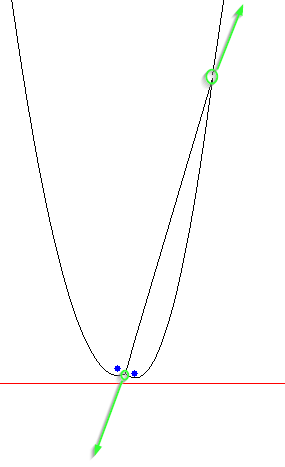
\includegraphics{ex77-counter}
    \caption{Counter example showing that the breakpoints on the beach line do not always move downwards.}
    \label{ex77:counter}
\end{figure}

If we have two points not directly over each other, as shown in \autoref{ex77:counter}, once the break points
occur, one will move downwards and one upwards.


\end{document}

